\documentclass[addpoints,spanish, 12pt,a4paper,cancelspace]{./include/gexam}

 %%%%%%%%%%%%%%%%%%%%%%%%%%%
 \renewcommand{\documentName} { Sistema de coordenadas cartesianos }
 \renewcommand{\documentContent} { \phantom{ } } 
 \renewcommand{\waterMark} { Modelo 7 } 

 % Configuración del documento.
 \renewcommand{\schoolSubject} { Examen Matemáticas 2º ESO  }
\renewcommand{\school} { IES José de Churriguera  }
\renewcommand{\academicPeriod} { Curso 2022/2023 }

\renewcommand{\autor} { Andrés Giménez Muñoz }
\renewcommand{\emailAuthor} { andresprofemates@outlook.es }
\renewcommand{\autorSing}{ Profesor: Andrés } 
 %%%%%%%%%%%%%%%%%%%%%%%%%%%
 
\renewcommand\subpartlabel{\thesubpart}
\renewcommand\subpartshook{\renewcommand\makelabel[1]{##1\hfil }} 
 
 %%%%%%%%%%%%%%%%%%%%%%%%%%%
 % Exam configuration
 %\pointsdroppedatright   %% No mostrar la puntuación
 \pointsinrightmargin{} % Para poner las puntuaciones a la derecha. Se puede cambiar. Si se comenta, sale a la izquierda.
 \extrawidth{-1.5cm} %Un poquito más de margen por si ponemos textos largos.
 \marginpointname{ \emph{\points}}
 
 %% Si se comenta no aparecerán los espacios de la solución.
 %\nocancelspace
 
 %% Puntuación a la izquierda.
%  \nopointsinrightmargin 

 %% Esto es de la clase exam. Si dejamos sin comentar \printanswers, se mostraran las soluciones. 
 %% Si la comentamos y dejamos sin comentar \noprintanswers, pues no se muestran las soluciones.
 % \printanswers
 %\noprintanswers
 
 %%%%%%%%%%%%%%%%%%%%%%%%%%%
 
 \begin{document}
 
%  \StudentData{}
%  \GradeTableHeader{}
 
 \justifying

% \begin{center}
%     \fbox{\fbox{\parbox{6.5in}{             
%                 \begin{itemize}
%                     \item Deben aparecer todas las operaciones, no vale solo con indicar el resultado.
%                     \item Se podrán quitar hasta cinco décimas por falta de claridad o rigor en el desarrollo de las respuestas o por una mala presentación.
%                     \item Se valorará que se indiquen las cuentas en línea, realizando las operaciones en el margen.
%                     \item No se puede utilizar la calculadora.
%                 \end{itemize}
%             }}}
% \end{center}
 
 \begin{questions}
    
    %% Gato
    \question Dibuja los puntos en el orden en el que aparece y únelos con segmentos de línea. \\
    \small

    Trazo 1: $(-9, -8)$ $(-14, -5)$ $(-15, -3)$ $(-15, -2)$ $(-15, -1)$ $(-15, 1)$ $(-14, 3)$ $(-13, 6)$ $(-13, 10)$ $(-12, 13)$ $(-11, 16)$ $(-8, 20)$ $(-7, 19)$ $(-7, 12)$ $(-8, 9)$ $(-9, 8)$ $(-8, 9)$ 
    $(3, 8)$ $(1, 7)$ $(3, 8)$ $(13, 11)$ $(18, 11)$ $(17, 10)$ $(12, 7)$ $(6, 5)$ $(4, 5)$ $(5, 5)$ $(5, -4)$ $(4, -5)$ $(3, -6)$ $(2, -7)$ $(0, -7)$
    
    Trazo 2:$(4, -5)$ $(4, -7)$ $(5, -9)$ $(6, -11)$ $(7, -11)$ $(8, -12)$ $(7, -13)$ $(9, -11)$ $(10, -11)$ $(10, -14)$ $(8, -18)$ $(7, -19)$ $(6, -19)$ $(6, -17)$ $(6, -19)$ $(-1, -19)$ 
    $(2, -15)$$(3, -12)$ $(3, -11)$ 
    
    Trazo 3:$(-1, -19)$ $(0, -20)$ $(-6, -20)$ $(-5, -19)$ $(-5, -14)$ $(-4, -10)$
    
    Trazo 4: $(-6, -11)$ $(-5, -14)$ $(-5, -19)$ $(-7, -20)$ $(-10, -20)$ $(-10, -19)$ $(-9, -18)$ $(-12, -14)$ $(-13, -11)$ $(-13, -9)$
    
    Trazo 5: $(-10, -19)$ $(-17, -19)$ $(-19, -16)$ $(-20, -13)$ $(-20, -12)$ $(-19, -11)$ $(-18, -11)$ $(-17, -13)$ $(-16, -16)$ $(-17, -13)$ $(-17, -12)$ $(-15, -11)$ $(-14, -9)$ 
    $(-13, -7)$ $(-13, -6)$
    
    Trazo 6:$(-11, -1)$ $(-10, -1)$ $(-9, -4)$ $(-7, -6)$ $(-6, -6)$ $(-4, -4)$ $(-3, -2)$ $(-3, -1)$ $(-2, -1)$ $(-4, -1)$ $(-6, 0)$ $(-8, 0)$ $(-9, -1)$ $(-11, -1)$
    
    Trazo 7: $(5, 1)$ $(10, 3)$ $(15, 4)$ $(20, 4)$ $(15, -4)$ $(8, -4)$ $(10, -9)$ $(6, -10)$ $(6, -11)$ $(5, -9)$ $(7, -8)$ $(5, -4)$
    
    Trazo 8: $(-15, 0)$ $(-14, 0)$ $(-13, -1)$ $(-13, -2)$ $(-14, -3)$ $(-15, -3)$ 
    
    Trazo 9: $(0, -2)$ $(1, -1)$ $(3, -1)$ $(4, -2)$ $(4, -3)$ $(3, -4)$ $(1, -4)$ $(0, -3)$ $(0, -2)$
    
    Trazo 10: $(-11, 1)$ $(-12, 2)$ $(-12, 3)$ $(-11, 4)$ $(-10, 4)$ $(-9, 3)$ $(-9, 2)$$(-10,1)$ $(-11, 1)$ 
    
    Trazo 11: $(-2, 2)$ $(-2, 3)$ $(-1, 4)$ $(0, 4)$ $(1, 3)$ $(1, 2)$ $(0, 1)$ $(-1, 1)$ $(-2, 2)$ 
    
    Trazo 12: $(-7, 1)$ 
    
    Trazo 13: $(12, 7)$ $(13, 11)$ 
    
    Trazo 14:$(-12, 13)$ $(-9, 15)$ $(-7, 15)$
    
    \normalsize

    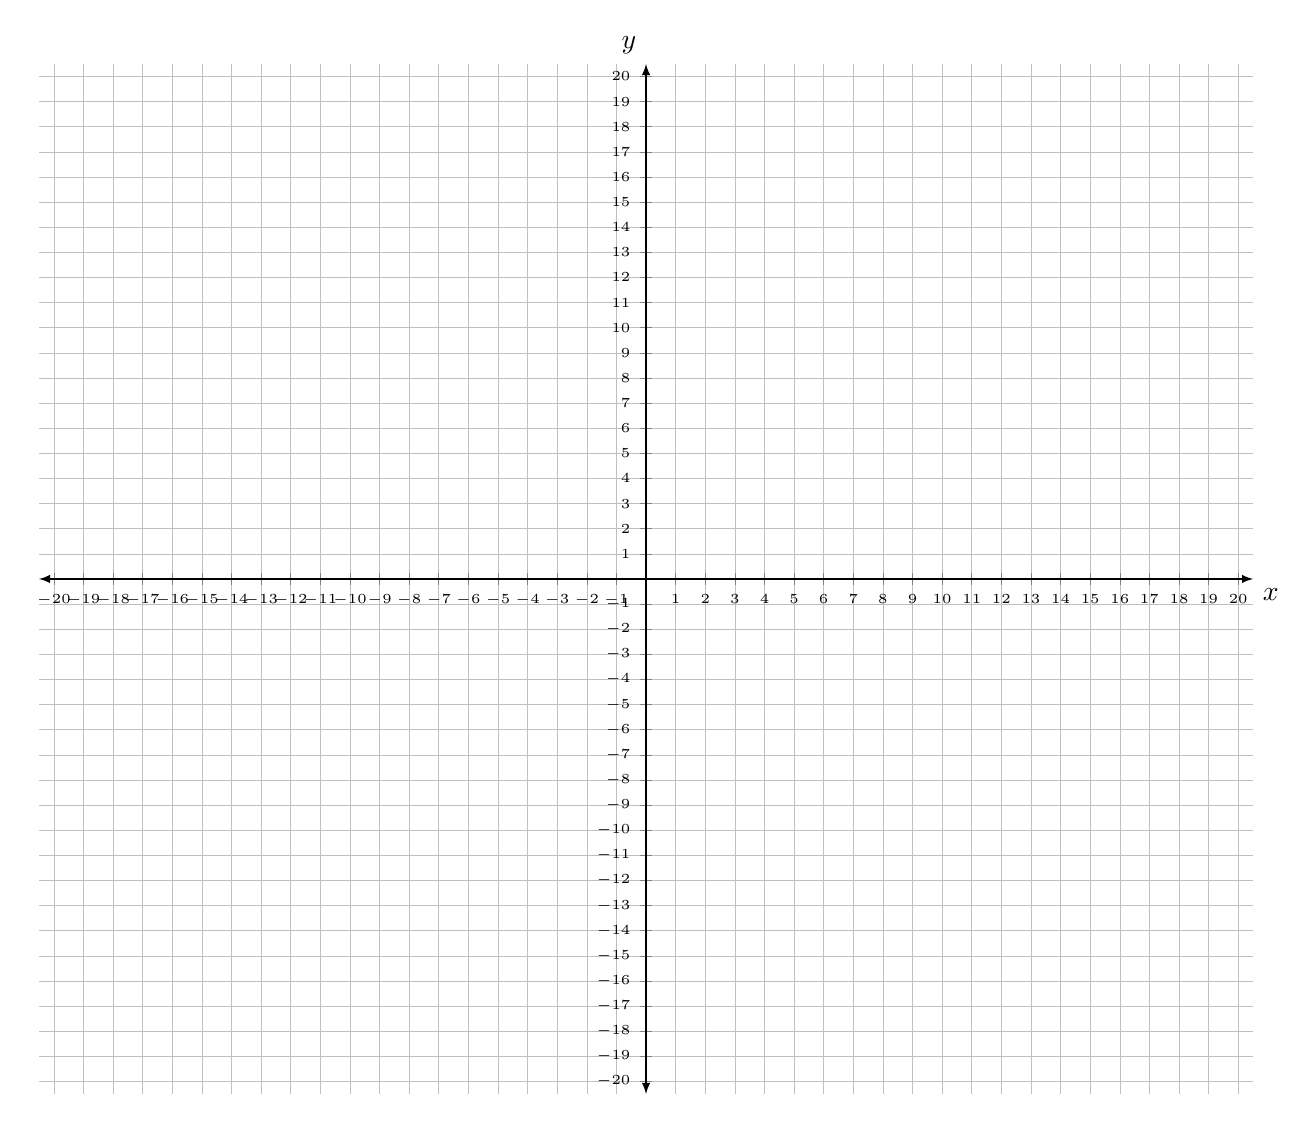
\begin{tikzpicture}[scale=1]
        \begin{axis}[
            axis x line=center,
            axis y line=center,
            xlabel = {$x$},
            ylabel = {$y$},
            xmin=-20,xmax=20,
            ymin=-20,ymax=20,
            xtick distance=1, 
            ytick distance=1, 
            grid=both,
            grid style={line width=.1pt, draw=gray!10},
            major grid style={line width=.2pt,draw=gray!50},
            axis lines=middle,
            axis line style={<->},
            minor tick num=0,
            enlargelimits={abs=0.5},
            axis line style={latex-latex},
            ticklabel style={font=\tiny},
            % ticklabel style={font=\tiny,fill=white},
            % xlabel style={at={(ticklabel* cs:1)},anchor=north west},
            % ylabel style={at={(ticklabel* cs:1$)},anchor=south west},
            xlabel style={below right},
            ylabel style={above left},
            width=17cm,
        ]
        
        \end{axis}

    \end{tikzpicture}

\end{questions}
 
\end{document}